%!TEX root = ../dissertation.tex
\begin{savequote}[75mm]
“A picture is worth a thousand swords.”
\qauthor{Tony}
\end{savequote}

\chapter{Reconstruction and Objects}

%%%%%%%%%%%%%%
\paragraph{}
Reconstruction is to reform the physics objects from raw detector readouts. 
In each pp collision recorded by ATLAS, charged particles bend and leave tracks in the ID, electrons and photons deposite their energy in ECAL, hadrons are abosrbed in HCAL, muons leave an extra track in the MS, and neutrinos are inferred by the conservation of momentum in the transverse plane. 
Figure~\ref{fig:reco_overview} gives an overview of the different sub-detectors that each type of particle will interact with in ATLAS.

\begin{figure}[h!]
  \centering
  \captionsetup{justification=centering}
  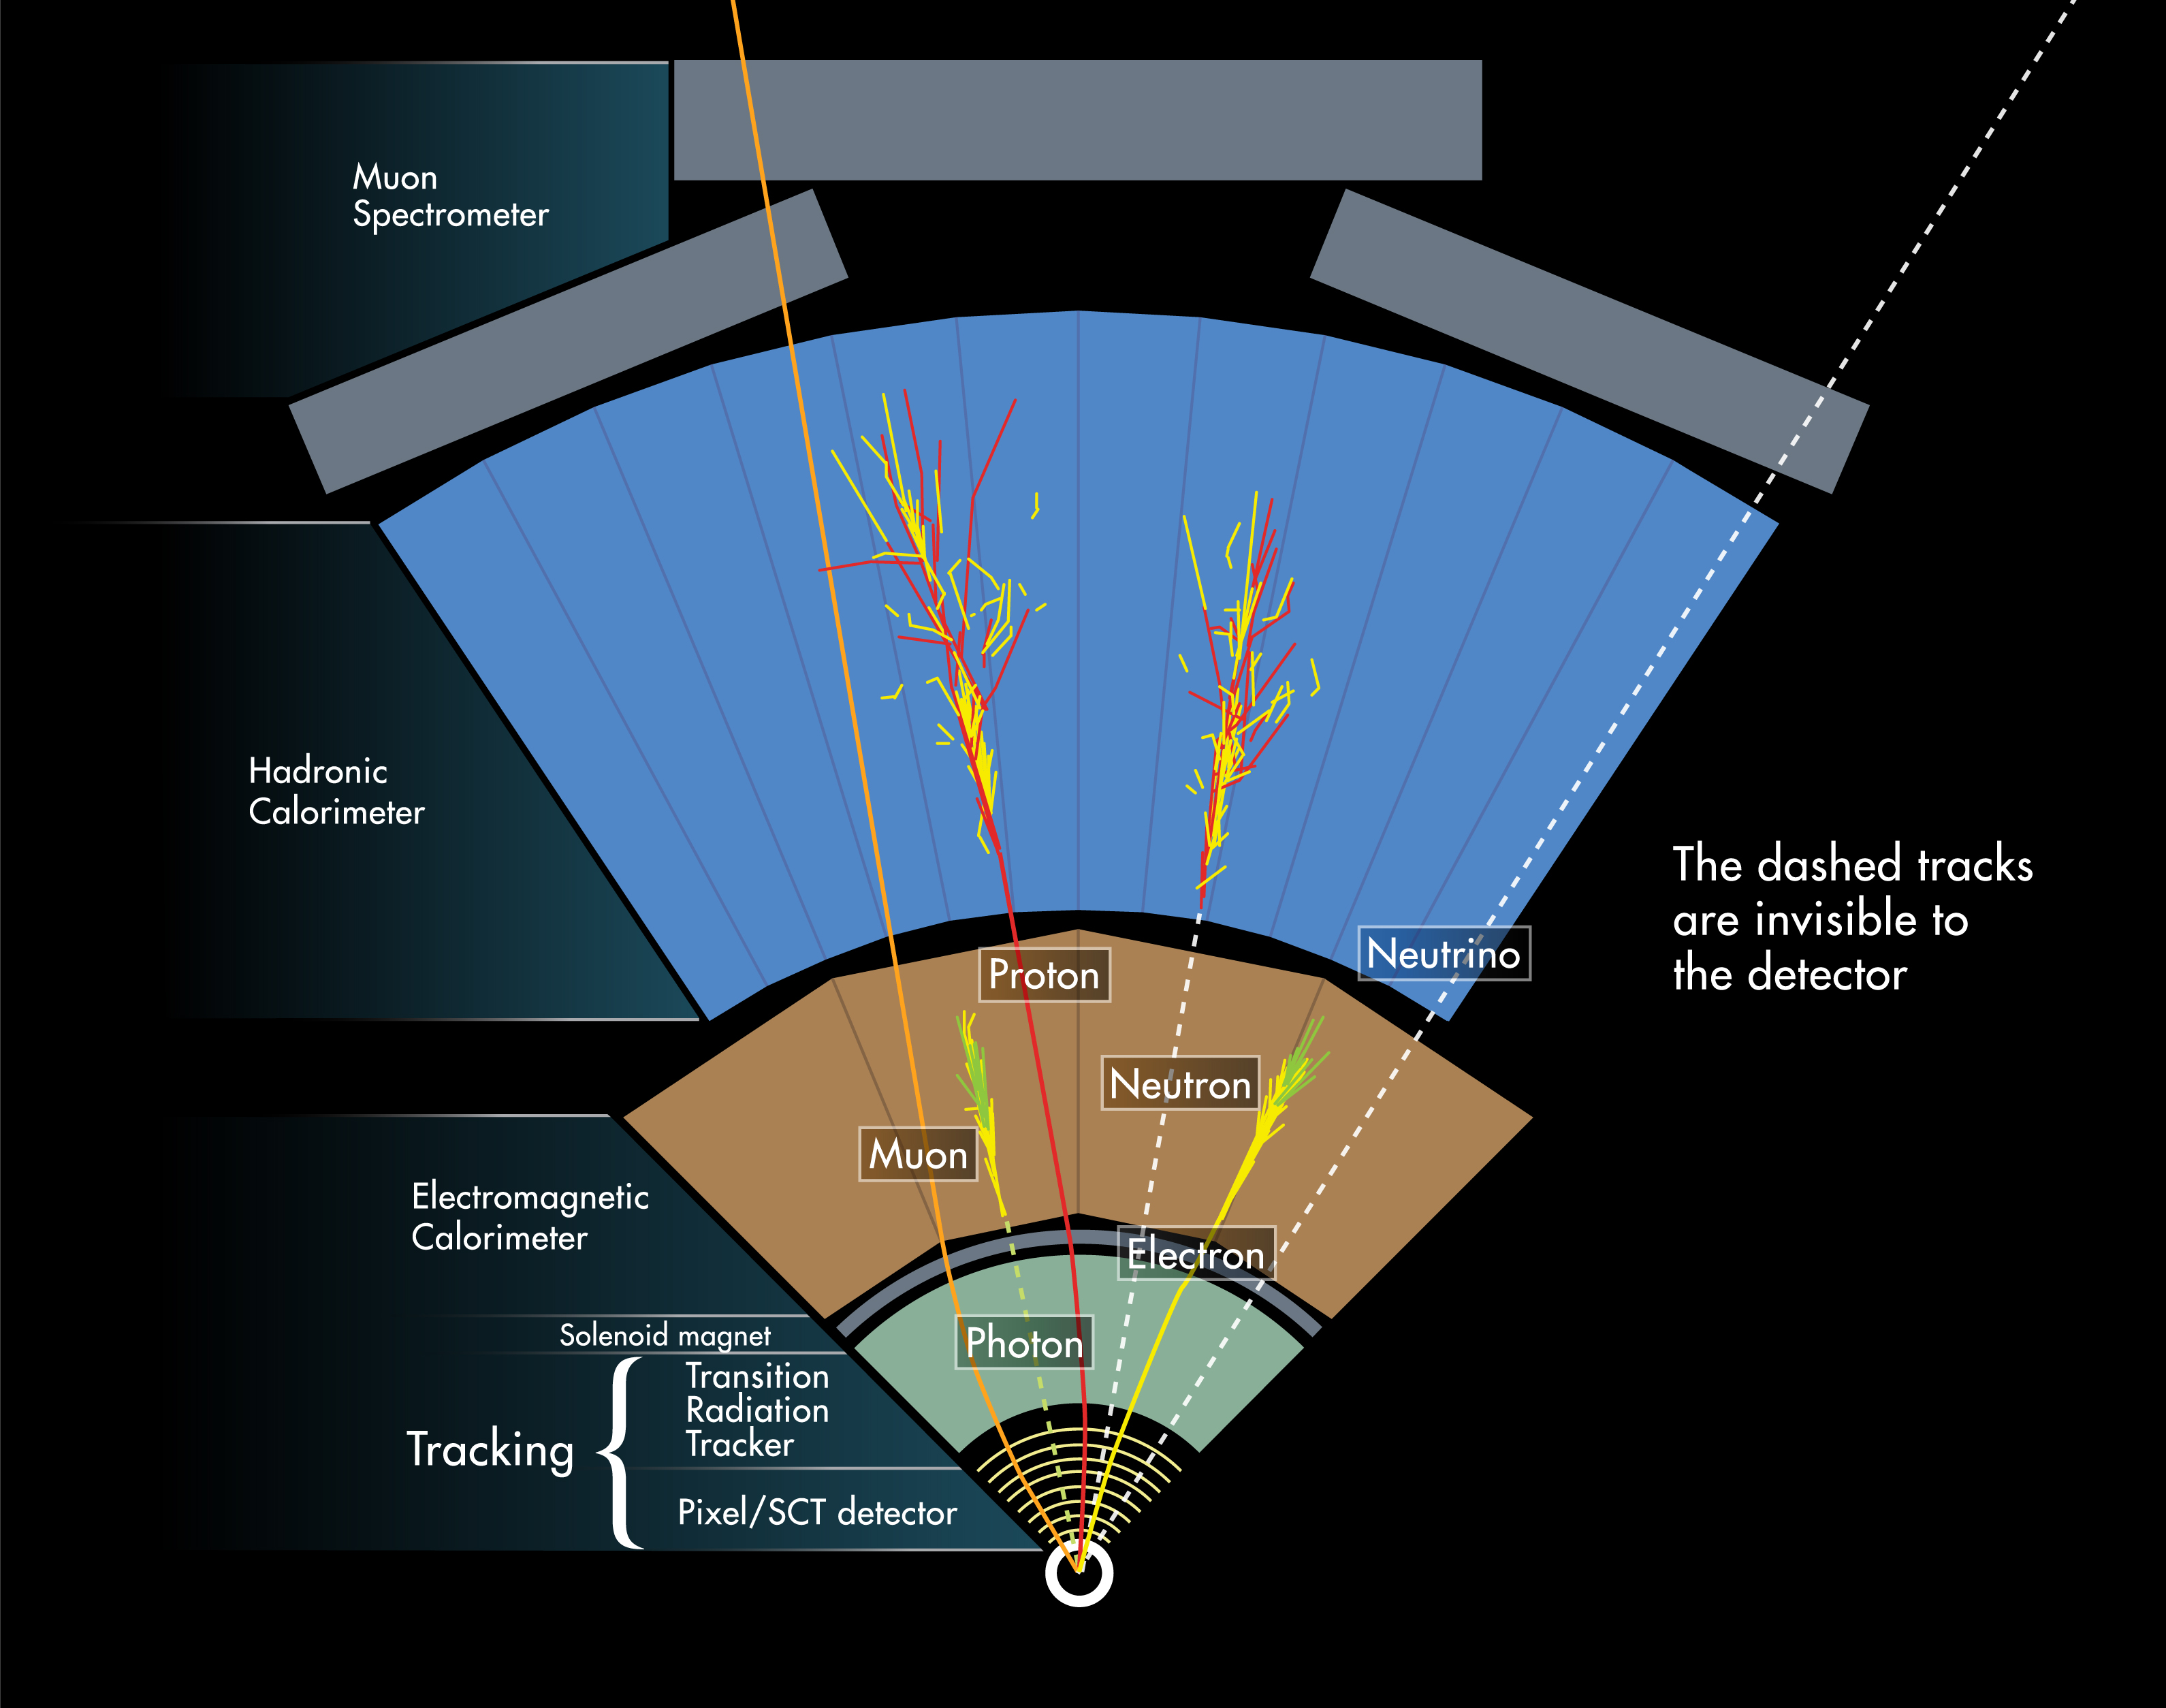
\includegraphics[width=0.6\textwidth]{figures/detector/ATLAS_particle}
   \caption{Illustration of particle interactions in ATLAS.}
  \label{fig:reco_overview}
\end{figure}

%%%%%%%%%%%%%%
\paragraph{}
Each pp collision generate multiple vertices, and they reconstructed from the available ID tracks. 
The primary vertex (PV), or the hard-scatter vertex, is selected as the one with the largest $\sum p_T^2$, where the sum is over all tracks with transverse momentum $p_T > 0.4$ \GeV that are associated with the vertex. 
Most physics objects are required to be consistent with the primary vertex.


%%%%%%%%%%%%%%
\section{Jets}
\paragraph{}
When a quark or gluon is produced in collisions, it produces a collimated spray of hadrons in the outcoming direction of the parton, which is known as a jet. 
Jets are built from topological clusters of energy deposits in calorimeter cells \cite{PERF-2014-07}, using a four-momentum reconstruction scheme with massless clusters as input. 
The directions of jets are corrected to point back to the primary vertex. 
Jets are reconstructed using the \akt algorithm with different values of the radius parameter \R. \R appears in the denominator of the clustering distance metric and determines the radial size of the jet in $\eta$-$\phi$ plane.

\subsection{Small-\R jets}
\paragraph{}
 The jets with $R=0.4$ (``small-\R jets'') are reconstructed from clusters calibrated at the electromagnetic (EM) scale. The jets are corrected for additional energy deposited from pile-up interactions using an area-based correction \cite{Cacciari:2008gn}. 
 They are then calibrated using \pt- and $\eta$-dependent calibration factors derived from simulation, before global sequential calibration~\cite{Aad:2011he} is applied, which reduces differences in calorimeter responses to gluon- or quark-initiated jets. 
 The final calibration is based on in situ measurements in collision data~\cite{ATL-PHYS-PUB-2015-015}.

 \paragraph{}
 ``small-\R jets'' are reuiqred to be consistent with the primary vertex, in order to avoid contamination from pileup interactions. 
 The jet vertex fraction (JVF) is the ratio of tracks associated with a primary vertex to the total number of tracks inside a jet. 
 Jets from the PV should have most tracks consistent with the PV and therefore have a large JVF value.
 %Jets with $p_T<60$~\GeV\, $|\eta|<2.4$, and with a large fraction of their energy arising from pile-up interactions are suppressed using tracking information, which was combined in a multivariate classification algorithm (\emph{jet vertex tagger})~\cite{ATL-PHYS-PUB-2014-001}. 
 %Events that pass a ``medium'' jet vertex tagger working point, corresponding to a 92\% efficiency for jets at the EM scale with $20<p_T<60$~\GeV, are retained in the analysis. 
 %Quality criteria are applied to the jets, and events with jets consistent with noise in the calorimeter or non-collision backgrounds are vetoed~\cite{jetcleanATLAS}.

\subsection{Large-\R jets}
\paragraph{}
The jets with $R=1.0$ (``large-\R jets'') are built from locally calibrated~\cite{Aad:2011he} topological clusters. They are trimmed~\cite{Krohn2010} to minimize the impact of energy deposits from pile-up interactions. 
Trimming proceeds by reclustering the jet with the \kt algorithm~\cite{Ellis:1993tq} into $R = 0.2$ subjets and then removing those subjets with $p_T^{\mathrm{subjet}}/p_T^{\mathrm{jet}} < 0.05$, where $p_T^{\mathrm{subjet}}$ is the transverse momentum of the subjet and $p_T^{\mathrm{jet}}$ that of the original jet. 
The energy and mass scales of the trimmed jets are then calibrated using \pt- and $\eta$-dependent calibration factors derived from simulation~\cite{PERF-2012-02}.


%Melissa asked me this question on Feb 13, 2017.
\paragraph{}
The calorimeter-based jet mass $m^{calo}$ for  a large-radius calorimeter jet $J$ is computed from the calorimeter cell cluster constituents $i$ with energy $E_i$ and momentum $p_i$:
\begin{equation}
m^{calo} = \sqrt{\left(\sum_{i\in J}E_i\right)^2-\left(\sum_{i\in J}\vec{p}_i\right)^2}.
\end{equation}

\paragraph{}
For a boosted massive particle, the angular spread in the decay products scales as $\frac{1}{p_T}$. 
For highly boosted cases, the spread could be comparable with the $\eta\time\phi \sim 0.1\time0.1$ calorimeter granularity. 
Tracking information can be used to maintain performance beyond this granularity limit.
The track-assisted jet mass, $m^{TA}$, is defined as:
\begin{equation}
m^{TA} = \frac{p_T^{calo}}{p_T^{track}} \cdot m^{track}.
\end{equation}
where $p_{T}^{calo}$ is the transverse momentum of the large-R calorimeter jet, $p_{T}^{track}$ is the transverse momentum of the four-vector sum of tracks associated to the large-R calorimeter jet, and $m^{track}$ is the invariant mass of this four-vector sum. This ratio corrects for charged-to-neutral fluctuations, and there improves the resolution with respect to track-only jet mass.

\paragraph{}
The two mass definitions are only weakly correlated with each other, therefore they can be linearily combined to the combined mass, $m^{comb}$, by weighting the components with $w$:
\begin{equation}
m^{comb} = w\cdot m^{calo}+(1-w)\cdot m^{TA}.
\end{equation}
The weight is determined for each large-R jet from the resolution functions of the calibrated track and calo mass terms.
This leads to a smaller mass resolution and better estimate of the median mass value than obtained using only calorimeter energy clusters, as shown in Figure~\ref{fig:Jet_mass}.

\begin{figure}[h!]
  \centering
  \captionsetup{justification=centering}
  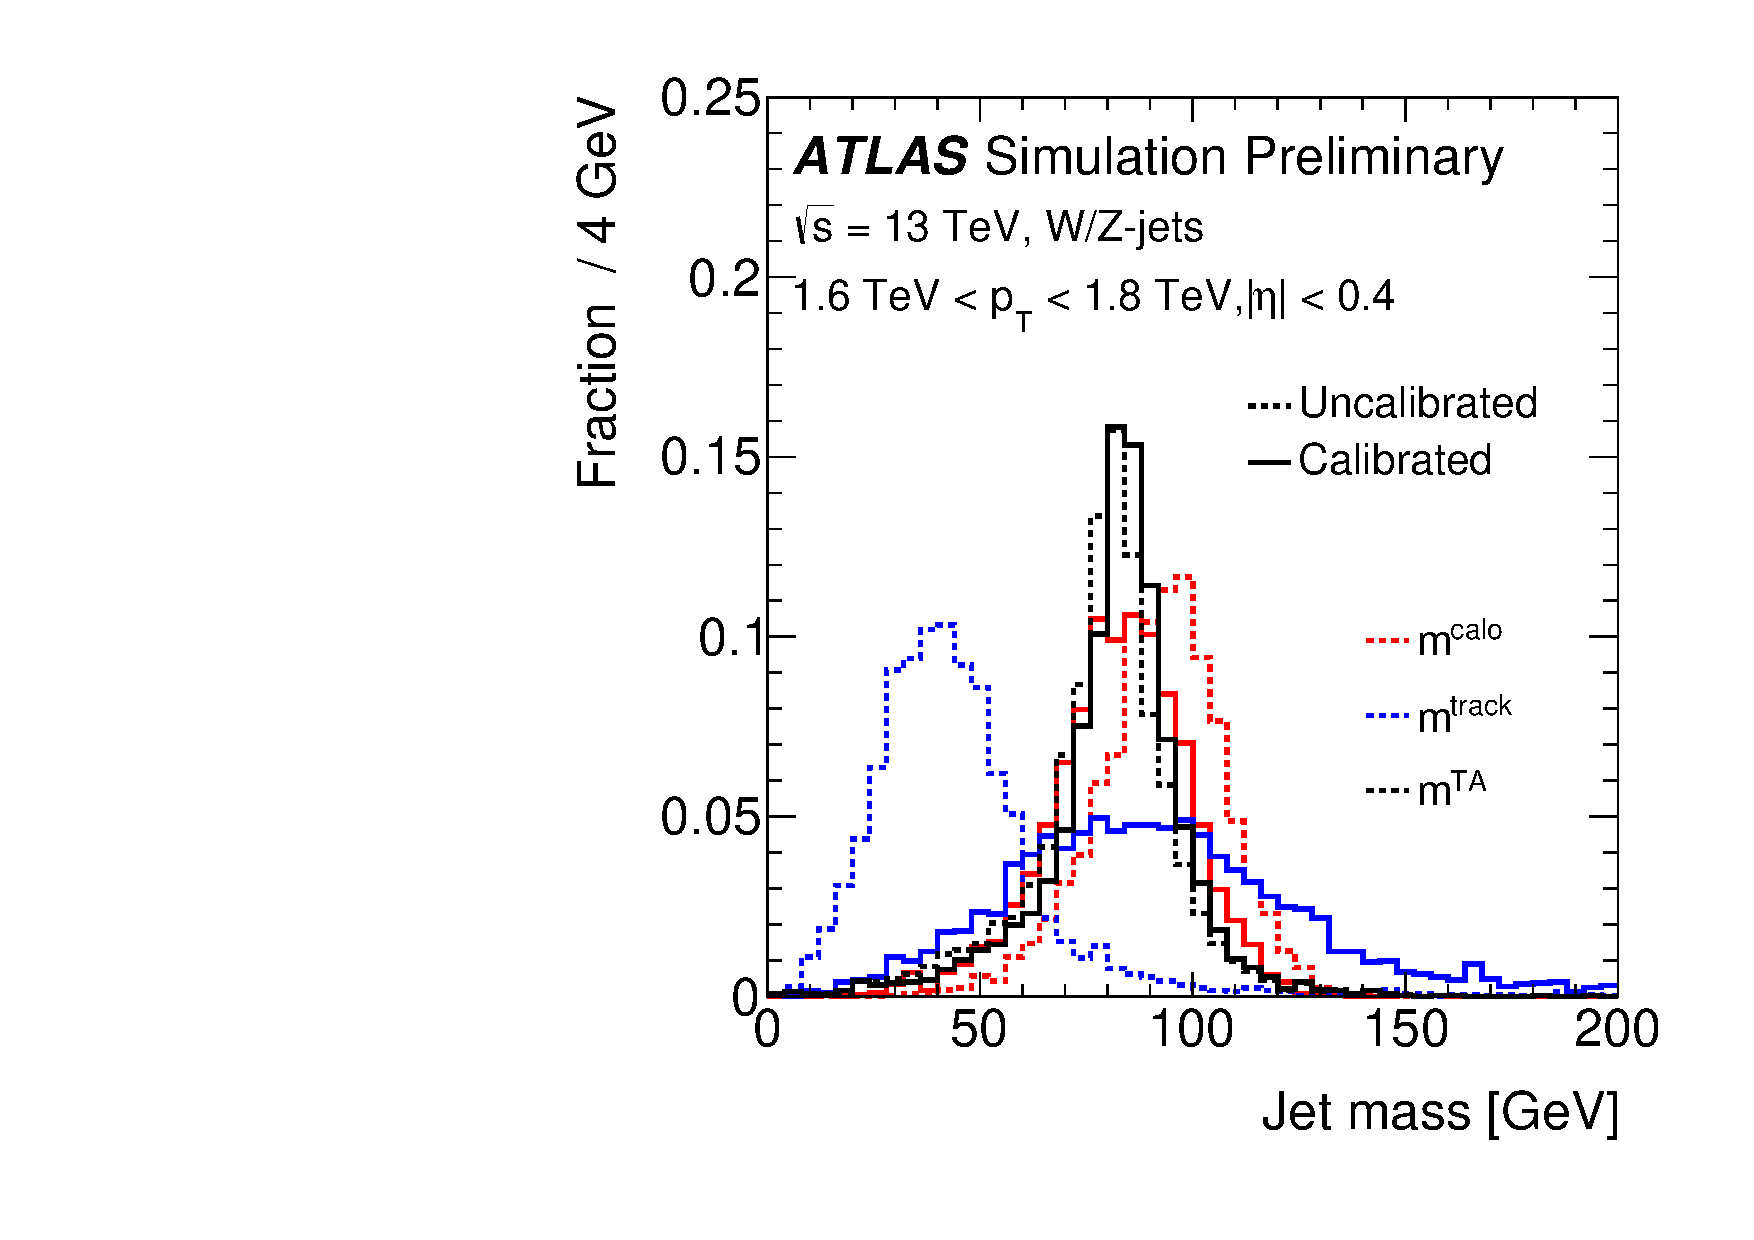
\includegraphics[width=0.5\textwidth,angle=-90]{figures/object/Jet_mass}
   \caption{Uncalibrated (dashed line) and calibrated (solid line) reconstructed jet mass distribution for calorimeter-based jet mass, mcalo (red), track-assisted jet mass mTA (black) and the invariant mass of four-vector sum of tracks associated to the large-radius calorimeter jet mtrack (blue) for W/Z-jets~\cite{ATLAS-CONF-2016-035}.}
  \label{fig:Jet_mass}
\end{figure}

%%%%%%%%%%%%%%
\section{Leptons}
\paragraph{}
Electron and photon identification is based on matching tracks to energy clusters in the ECAL and relying on the longitudinal and transverse shapes of the EM shower~\cite{ATLAS-CONF-2016-024}. Well-reconstructed ID tracks matched to clusters are classified as electron candidates, while clusters without matching tracks are classified as unconverted photon candidates. Clusters matched to a reconstructed conversion vertex or to pairs of tracks consistent with the conversion hypothesis are classified as converted photon candidates. Eletrons and photons are not used in this thesis.

\paragraph{}
Hadronic tau decays are composed of a tau neutrino and one or three charged pions and up to two neutral pions~\cite{ATLAS-CONF-2017-029}. The tau reconstruction is seeded by jets, and matched one or three associated tracks, with a total electric charge of $\pm 1$. A Boosted Decision Tree (BDT) identification procedure, based on calorimetric shower shapes and tracking information is used to reject backgrounds from jets. Hadronic taus are not used in this thesis.

\paragraph{}
Neutrinos are infered from the missing transverse momentum (MET), or $E_T^{miss}$. Neutrios do not interact with the ALTAS. Their presence can only be deduced from the conservation of transverse momentum in each collison, as the incoming protons have no net momentum in the transverse plane. MET is calculated as the negative vectorial sum of the \pt of all fully reconstructed and calibrated physics objects. This procedure includes a “soft term”, which is calculated using the ID tracks that originate from the primary vertex but are not associated with reconstructed objects. MET is not used in this thesis.

\paragraph{}
Muons are identified by matching ID tracks with reconstructed MS tracks~\cite{Aad:2016jkr}. For this thesis, muons must have $p_T > 4~\GeV$, $|\eta| < 2.5$ and to satisfy ``medium'' muon identification criteria~\cite{PERF-2015-10}. If a muon is within $\DR = 0.4$ (0.2) of a jet used for $b$-tagging in the resolved (boosted) analysis, their four-momentum is added to the calorimeter-based jet's four-momentum to partially account for the energy lost in semileptonic $b$-hadron decays. 

%%%%%%%%%%%%%%
\section{Flavor Tagging}
\paragraph{}
Tracks reconstruction, see \href{https://cds.cern.ch/record/2254947/files/PERF-2015-08-002.pdf}{this great note}. The first step is creating clusters based on pixel and SCT meausred energy deposits, which are space-points. Then three space-points form a seed, and tey are cobmined to build track candidates using a Kalman filter. After ambiguity solving, an artificial neural network is trained and used to identy merged clusters. The last step is a high resolution fit, which is CPU intensive. The min $p_T$ is 400 MeV, and $|\eta| < 2.5$, and at least seven hits in the pixel or SCT. Total number of holes has to be less than two per track, and no more than one in the pixels. $Z_{0}^{BL} \sin{\theta}$ is requred to be less than 3 mm. Interestingly, the performance of track reconstruction is highly dependent on the momentum of the particle. With higher boost, the decay tracks have smaller seperations in the inner detector, hindering the resolving cluster process, and thus degrading the track identification efficiency. For a 1 TeV $B_{0}$, the reconstruction track effieincy is $83\%$, compared to $95\%$ for a 200 GeV $B_{0}$.

\paragraph{}
$b$-tagging. see \href{https://cds.cern.ch/record/2160731/files/ATL-PHYS-PUB-2016-012.pdf}{2016 run2 note}. Recurrent Neural Network(RNN), which could explore more the correlation between different input parameters, especially the fragmentagion of jets and the impact parameters, has shown improvements in $b$-tagging efficiency and is under investigation for future Multivariate Taggers, see \href{https://cds.cern.ch/record/2253371}{RNN note}. $b$-jet calibration is done using $t\top{t}$ events, as can be seen in \href{https://indico.cern.ch/event/622490/contributions/2510894/attachments/1425202/2191220/ttbar_PDF_Calibration_MVA_Training_Approval_140317.pdf}{Likelihood talk} and \href{https://cds.cern.ch/record/1538335/files/ATL-COM-PHYS-2013-395.pdf}{Matrix method and Likelihood note} or a Tag-and-Probe using semi-leptonic $t\top{t}$ events.

\paragraph{}
There are 3 taggers in MV2 family, MV2c00, MV2c10, MV2c20 depending on their charm composition in training: $MV2c00->0\%$ c-fraction in the training, $MV2c10->7\%$ c-fraction in the training and $MV2c20->15\%$ c-fraction in the training. See \href{https://twiki.cern.ch/twiki/bin/view/AtlasProtected/BTaggingMV2}{twiki}.

\paragraph{}
Vertex reconstruction and resolution, can be seen in this \href{http://atlas.web.cern.ch/Atlas/GROUPS/PHYSICS/PUBNOTES/ATL-PHYS-PUB-2015-026/}{note}. Track resolution can be seen in this \href{https://cds.cern.ch/record/2110140/files/ATL-PHYS-PUB-2015-051.pdf}{note}. In Run2, the $d_0$ resolution is about 10 $\mu m$ and $z_0$ is about $50 \mu m$, both decreases as a function of track momentum.

\paragraph{}
The increase of tracks from fragmentation in the high jet $p_T$ region is the main reason for the performance degradation. As the jet $p_T$ increases, the number of fake vertices is increasing, while the secondary vertex reconstruction effieincy for b and c jets slighly decreases with jet $p_T$.

\paragraph{}
See the reference \href{https://twiki.cern.ch/twiki/bin/viewauth/AtlasProtected/BTaggingPaperRecommendations}{here}. Operating points are defined by a single cut value on the discriminant output distribution and are chosen to provide a specific b-jet efficiency on an inclusive ttbar sample. The $77\%$ working point has a rejection factor of 6 and of 134 on charm and light-jets, respectively. (More information on the working points can be extracted from Table 2 and the related section in ATL-PHYS-PUB-2016-012).

\paragraph{}
Correction factors are applied to the simulated event samples to compensate for differences between data and simulation in the b-tagging efficiency for b, c and light-jets. The correction for b-jets is derived from ttbar events with final states containing two leptons, and the corrections are consistent with unity with uncertainties at the level of a few percent over most of the jet pT range.

\paragraph{}
Uncertainties on the correction factors for the b-tagging identification response are applied to the simulated event samples by looking at dedicated flavour-enriched samples in data. An additional term is included to extrapolate the measured uncertainties to the \textbf{high-pT} region of interest. This term is calculated from simulated events by considering variations on the quantities affecting the b-tagging performance such as the impact parameter resolution, percentage of poorly measured tracks, description of the detector material, and track multiplicity per jet. The dominant effect on the uncertainty when extrapolating to high-pT is related to the different tagging efficiency when smearing the track impact parameters based on the resolution measured in data and simulation.


%Although this work doesn't depend on specific boosted W/Z/H/Top taggers, many analysises adopt them and improve search sensitivities. For machine learning techiniques applied, see this \href{https://cds.cern.ch/record/2242830/files/ATL-COM-PHYS-2017-031.pdf}{W/Top tagger using BDT/DNN}

